%\RequirePackage[]{optional}
%\RequirePackage[slides]{optional}
\RequirePackage[notslides]{optional}

\opt{slides}{
% Following for presentation mode
\documentclass[10pt]{beamer}
\usepackage{xmpmulti}
%usetheme{Berlin}
}
\opt{notslides}{
% Following for notes mode
\documentclass[a4paper]{article}
\usepackage{beamerarticle}
\usepackage{a4wide}
\usepackage{graphicx}
\usepackage{amsfonts}
\usepackage{fancyhdr}
}

% Following for all modes
%\usepackage{auto-pst-pdf}
%\usepackage{pst-pdf}
\usepackage{psfrag}

\parindent=0ex
\parskip=1ex
\newcommand{\conv}{\ast}
\reversemarginpar

%\title{Fourier series}
%\author{}
%\date{}

\begin{document}
\pagestyle{fancy}
\fancyhead{}
\renewcommand{\headrulewidth}{0pt}
\fancyfoot[C]{\thesection-\thepage}
%\fancyfoot[R]{fcn2010}

\begin{frame}
\titlepage
\end{frame}

\setcounter{section}{3}
\section{Fourier series}

%\mode<article>{{\bf \LARGE The Fourier series}}

%NOTE:  BARANUIK NOTES ON CONNEXIONS HAS NICE INTRO STUFF
%NICE DETAILS ON SUPERPOSITION INTEGRAL:  http://cnx.org/content/m27499/latest/

Any LTI system is completely determined by its impulse response $h(t)$.  This is the output of the system when the input is a Dirac delta function at the origin.  In linear systems theory we are usually more interested in how a system responds to signals at different frequencies.  When we talk about a signal of frequency $\omega$, we mean the signal $e^{j \omega t}$.  This is the {\em only} signal that will contain both a $t$ variable and a $\omega$ variable in its specification --- it defines the relationship between the time and frequency domains.  Note that $j = \sqrt{-1}$, so the signal is complex valued.

The pertinent question is this:  what happens to a pure frequency when it passes through a particular linear system?  Assuming the input is $x(t) = e^{j \omega t}$, and assuming that the frequency $\omega$ is fixed at some value of interest, the output is simple to derive from convolution:
\begin{align*}
  y(t) &= \int_{-\infty}^{\infty} h(\tau) x(t-\tau) d\tau = \int_{-\infty}^{\infty} h(\tau) e^{j \omega (t-\tau)} d\tau
  = \int_{-\infty}^{\infty} h(\tau) e^{-j \omega \tau} e^{j \omega t} d\tau \\
  &= \left( \int_{-\infty}^{\infty} h(\tau) e^{-j \omega \tau} d\tau \right) e^{j \omega t} 
  = H(\omega) e^{j \omega t}.
\end{align*}
Since $\omega$ is fixed, $H(\omega)$ is a number, possibly complex valued, that depends on the impulse response $h(t)$.  We see that the system therefore has the following input-output pair:
\begin{equation*}
  e^{j \omega t} \longrightarrow H(\omega) e^{j \omega t}.
\end{equation*}
Looking at it differently, if the input-output relation of the system is written as $y(t) = T\{x(t)\}$, then the complex exponential input satisfies the property
\begin{equation*}
  T \left\{ e^{j \omega t} \right\} = H(\omega) e^{j \omega t}.
\end{equation*}
This is an eigen relation:  the transformation $T$ applied to the signal $e^{j \omega t}$ results in the same signal $e^{j \omega t}$, but multiplied by a constant $H(\omega)$ that depends on the frequency $\omega$ and is determined by the system.  Complex exponential functions (or pure frequencies) are characteristic functions for LTI systems:  they propagate through without change, except for an overall (complex) scaling.  For any given system the scaling depends on the frequency of the complex exponential.  Alternatively, LTI systems cannot create frequencies at the output that were not already present at the input:  they can only modify them by a complex-valued scaling.

\begin{center}
\fbox{
\begin{minipage}{0.9\textwidth}
The function
\begin{equation*}
  H(\omega) = \int_{-\infty}^{\infty} h(\tau) e^{-j \omega \tau} d\tau
\end{equation*}
is called the {\em frequency response} of the system.  For any value of $\omega$ it tells us how the system responds to an input frequency $e^{j \omega t}$:  the output will be $H(\omega) e^{j \omega t}$.  If you know the impulse response $h(t)$ of a system, then you also know its frequency response $H(\omega)$ from the formula given.  The quantity $H(\omega)$ is also called the {\em transfer function} of the system.
\end{minipage}
}
\end{center}

The Fourier series decomposition allows us to express any {\em periodic} signal $x(t)$ with period $T$ as a linear combination (or weighted sum) of a countable set of frequencies:
\begin{equation*}
  x(t) = \sum_{k={-\infty}}^{\infty} c_k e^{j k \omega_0 t}
\end{equation*}
for some coefficients $c_k$.  Putting this signal through an LTI system is simple:  the output is
\begin{align*}
  y(t) &= T \{x(t)\} = T \left\{ \sum_{k={-\infty}}^{\infty} c_k e^{j k \omega_0 t} \right\} 
  = \sum_{k={-\infty}}^{\infty} c_k T \left\{ e^{j k \omega_0 t}  \right\} \\
  &= \sum_{k={-\infty}}^{\infty} c_k H(k \omega_0) e^{j k \omega_0 t}
  = \sum_{k={-\infty}}^{\infty} d_k e^{j k \omega_0 t},
\end{align*}
with $d_k = c_k H(k \omega_0)$.  The transformation of coefficients $d_k = c_k H(k \omega_0)$ tells us exactly how the different frequency components in the signal are affected by the system.  Thus if we can get used to thinking about signals in the frequency domain, we have a very simple way of interpreting the action of LTI systems on signals.

Complex exponential are the eigenfunctions of LTI systems:  they are the only functions that propagate through linear systems without change except for multiplication by a complex scale factor.  Coupled with the fact that any periodic signal can be expressed as a weighted sum of a set of complex exponentials, this gives a very intuitive description of a system:  inputs are linear combinations of complex exponentials, and outputs are linear combinations of responses to complex exponentials.  The weights in the linear combinations at the output are related to the weights at the input by multiplication with the system transfer function $H(\omega)$.

Most signals in the world are real.  It may seem strange to express a real-valued signal as a linear combination of complex signals.  Nonetheless, the truth of the matter is that it makes things simpler, both in terms of understanding and in terms of algebra.  Complex exponentials are the natural building blocks of signals, even though we're usually only interested linear combinations of complex exponentials that end up being real valued.

\subsection{Complex numbers:  a review}

Letting $j = \sqrt{-1}$ we can write a complex number in two ways:
\begin{itemize}
\item Rectangular form:  
\begin{align*}
  s = a + jb, \qquad & a = \text{Re}(s) \quad \text{(real part)} \\
  & b = \text{Im}(s) \quad \text{(imaginary part)}
\end{align*}
\item Polar form:
\begin{align*}
  s = \rho e^{j \theta}, \qquad & \rho = |s| \quad \text{(nonnegative magnitude)} \\
  & \theta = \angle s \quad \text{(phase)}.
\end{align*}
\end{itemize}

Euler's formula states that
\begin{equation*}
  e^{j \theta} = \cos(\theta) + j \sin(\theta)
\end{equation*}
and links these two representations algebraically.  This can be used directly to convert a complex number from polar to rectangular form:
\begin{equation*}
  s = \rho e^{j \theta} = \rho (\cos(\theta) + j \sin(\theta))
  = \rho \cos(\theta) + j \rho \sin(\theta) = a + j b,
\end{equation*}
with $a = \rho \cos(\theta)$ and $b = \rho \sin(\theta)$.  To covert from rectangular to polar form we note that
\begin{equation*}
  a^2 + b^2 = \rho^2 \cos^2(\theta) + \rho^2 \sin^2(\theta) = \rho^2 (\cos^2(\theta) + \sin^2(\theta)) = \rho^2
\end{equation*}
and 
\begin{equation*}
  b/a = \frac{\sin(\theta)}{\cos(\theta)} = \tan(\theta),
\end{equation*}
so the magnitude and phase components of the complex number are given by
\begin{align*}
  \rho &= \sqrt{a^2 + b^2} \\
  \theta &= \begin{cases}
    \arctan(b/a) \qquad & a \geq 0 \\
    180^\circ + \arctan{-1}(b/a) \qquad & a < 0.
  \end{cases}
\end{align*}

These representations are linked very naturally via the correspondence of complex numbers with the 2D plane, also called the {\em Argand diagram}:
\begin{center}
  \psfrag{s=a+jb}{\scriptsize $s = a + j b$}
  \psfrag{a}{\scriptsize $a$}
  \psfrag{b}{\scriptsize $b$}
  \psfrag{|s|}{\scriptsize $|s|$}
  \psfrag{as}{\scriptsize $\angle s$}
  \includegraphics{complexnumberplane}
\end{center}

Doing algebra on complex numbers is easy as long as they are expressed in the appropriate form.  Defining the two complex numbers $s_1$ and $s_2$ according to
\begin{equation*}
  s_1 = a_1 + j b_1 = \rho_1 e^{j \theta_1} \qquad \text{and} \qquad 
  s_2 = a_2 + j b_2 = \rho_2 e^{j \theta_2},
\end{equation*}
the following operations are simple:
\begin{itemize}
\item Addition:  $s_1 + s_2 = (a_1 + j b_1) + (a_2 + j b_2) = (a_1 + a_2) + j (b_1 + b_2)$
\item Subtraction:  $s_1 - s_2 = (a_1 + j b_1) - (a_2 + j b_2) = (a_1 - a_2) + j (b_1 - b_2)$
\item Multiplication:  $s_1 s_2 = (\rho_1 e^{j \theta_1}) (\rho_2 e^{j \theta_2}) = \rho_1 \rho_2 e^{j (\theta_1 + \theta_2)}$
\item Division:  $s_1/s_2 = (\rho_1 e^{j \theta_1}) (\rho_2 e^{j \theta_2})^{-1} = (\rho_1/\rho_2) e^{j (\theta_1 - \theta_2)}$.
\end{itemize}
To add or subtract two complex numbers, express them in rectangular form and the operation follows.  To multiply or divide complex numbers, use polar forms.  Note that as far as algebra is concerned you can think of $j$ as a normal variable --- it just happens to have a value of $\sqrt{-1}$.

Consider a plot of the function $x(t) = \sin(2 \pi t)$, expressed in polar form.  The signal $x(t)$ is shown below, along with $|x(t)|$ and $\angle x(t)$:
\begin{center}
  \psfrag{pi}{$\pi$}
  \psfrag{-pi}{$\!\!\!-\pi$}
  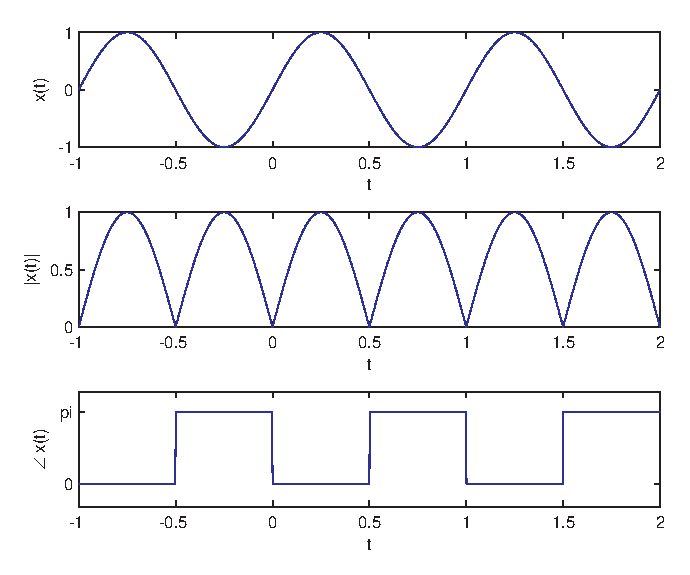
\includegraphics{sinmagphase}
\end{center}
Note that, even though the signal is real, the phase is {\em nonzero}.  This becomes obvious if you plot the number $-1$ on the Argand diagram:  
\begin{center}
  \psfrag{pi}{\scriptsize $\pi$}
  \includegraphics{sinmagphasead}
\end{center}
Evidently when expressed in polar form we have $-1 = 1 e^{j \pi}$, which has a magnitude of $1$ and a phase of $\pi$.  The same is true for any negative real number:  it has a phase of $\pi$, because the magnitude must be positive.  

However, note also that $-1 = 1 e^{-j \pi}$ --- we're just measuring the angle in the negative direction instead of the positive direction.  Phase is not determined up to addition by a multiple of $2 \pi$:  a phase of $0.3$ radians is equivalent to a phase of $0.3 + 2 \pi$ radians or $0.3 + (2) 2 \pi$ radians or $0.3 - 2 \pi$ radians --- we're just going around the unit circle by multiples of a full circle, but the point in the Argand diagram (and hence the corresponding complex number) is unchanged.  Thus, in the plot of $\angle x(t)$ we could have given the portions of the signal indicated with the value $\pi$ the value $\pi + k (2 \pi)$ for any integer $k$.  Positive real numbers have phases of $0, \pm 2\pi, \pm 4\pi, \dots$;  negative real numbers have phases of $\pm \pi, \pm 3\pi, \ldots$.

\subsection{Fourier series formulation}

Suppose we are given a signal $x_s(t)$, which can be a real or complex valued function of a (real) time variable $t$. Furthermore, suppose that the signal is periodic with period $T$:  for all $t$ we have $x_s(t) = x_s(t + T)$. 

We define the (parametric) signal $x(t)$ to be the weighted sum of an infinite set of complex exponentials
\begin{equation*}
  x(t) = \sum_{k=-\infty}^\infty a_k e^{j (2\pi k/T) t},
\end{equation*}
for some given set of coefficient weights $\{a_k\}_{k=-\infty}^\infty = \{ \ldots, a_{-1}, a_0, a_1, \ldots \}$.  Note that we allow these coefficients to be complex numbers, and in general the function $x(t)$ can be complex valued.  We can describe the relation above by saying that $x(t)$ can be written as a {\em linear combination} or {\em weighted sum} of complex exponential signals $e^{j (2\pi k/T) t}$.  The weights of each complex exponential are the values $a_k$ in the summation.

We will not prove it in this course, but if $x_s(t)$ is sufficiently well behaved (like all real-world signals are), then we can always find a set of coefficients $a_k$ for $k \in \mathbb{Z}$ such that $x(t)$ is {\em almost exactly}\footnote{Almost exactly in this context means that for any $\epsilon > 0$ we can find a set of coefficients $a_k$ such that 
\begin{equation*}
  \int_0^T |x(t) - x_s(t)|^2 dt < \epsilon.
\end{equation*}
This means that the difference in the energy of the two signals is arbitrarily small, but does not necessarily mean that $x(t) = x_s(t)$ for all $t$.  (The difference between these two statements is quite subtle, and unimportant for most practical purposes.)} equal to $x_s(t)$.  

The periodic signal $x(t)$ can be completely described by the set of values that it takes for $0 \leq t < T$.  Formally, to know $x(t)$ we just need to know all values of the (infinite) set $\{x(t)|t \in \mathbb{R}, 0 \leq t < T\}$ (the set of values of $x(t)$ such that $t$ is real and $0 \leq t < T$).  From the previous assertion $x(t)$ can alternatively be described by the set of coefficients $a_k$ for $k \in \mathbb{Z}$, or the elements of the (infinite) set $\{a_k|k \in \mathbb{Z}\}$ (the set of values of $a_k$ such that $k$ is any integer).  For our purposes these two descriptions are {\em exactly equivalent}:  if $a_k$ for $k \in \mathbb{Z}$ are specified then $x(t)$ is completely determined, and any $x(t)$ corresponds to a set of coefficients $a_k$ that completely describes it.  

The important (basis) functions in the Fourier series representation are the complex exponentials with frequencies $\omega_k = \frac{2 \pi k}{T}$, for integer $k$ (positive or negative).  There are an infinite number of these complex exponential functions:
\begin{equation*}
  \ldots, e^{-j \frac{4 \pi}{T} t}, e^{-j \frac{2 \pi}{T} t}, e^{j 0 t}, e^{j \frac{2 \pi}{T} t}, e^{j \frac{4 \pi}{T} t}, \ldots,
\end{equation*}
corresponding to frequencies $\ldots, -\frac{4 \pi}{T}, -\frac{2 \pi}{T}, 0, \frac{2 \pi}{T}, \frac{4 \pi}{T}, \ldots$.  Each of these functions can be regarded as a complex-valued signal.  In the Fourier series representation each of these complex exponentials is assigned a weight, and the sum of all of the weighted complex exponentials yields the desired signal.

People (especially engineers) will often talk about the "amount" of a frequency present in a signal:  by this they mean some quantity related directly to the coefficient weighting the complex exponential at that frequency.  The fact that the Fourier series representation for a periodic signal with period $T$ exists leads to the interesting observation that such a signal {\em only} contains frequencies at integer multiples of $\omega_0 = \frac{2 \pi}{T}$.  This is the {\em fundamental frequency} of the signal, expressed in radians per second.

The Fourier series representation is constructed as the sum of an infinite set of products of the form $a e^{j \omega t}$, where $a$ is generally complex.  It is really worth understanding how multiplication by $a$ affects the complex exponential $e^{j \omega t}$.  First of all let's think of a specific complex exponential signal $x(t) = e^{j \omega_0 t}$ at some frequency $\omega_0$.  Note that $x(t) = e^{j \omega_0 t} = 1 e^{j \omega_0 t}$ is a complex-valued function, expressed in polar form.  Thus the magnitude is $|x(t)| = 1$, a constant function, and the phase is $\angle x(t) = \omega_0 t$.  

Now consider the signal $y(t) = a x(t)$, where $a$ is a constant.  The right hand side involves multiplication of complex quantities, so we should write $a$ in polar form:  $a = \rho e^{j \phi}$.  Then
\begin{equation*}
  y(t) = a x(t) = \rho e^{j \phi} e^{j \omega_0 t} = \rho e^{j (\omega_0 t + \phi)} 
\end{equation*}
which is also a complex valued function in polar form:  $|y(t)| = \rho$ and $\angle y(t) = \omega_0 t + \phi$.  Comparing the representations we see that multiplication by $a$ changes the magnitude of the complex exponential by $|a|$, and adds an overall phase of $\angle a$.

To really see the effect, we can note that $y(t)$ can be written in terms of $x(t)$ as
\begin{equation*}
  y(t) = \rho e^{j (\omega_0 t + \phi)} 
  = \rho e^{j \left( \omega_0 \left( t + \frac{\phi}{\omega_0} \right) \right)}
  = \rho x \left( t + \frac{\phi}{\omega_0} \right).
\end{equation*}
(This is only true if $x(t) = e^{j \omega_0 t}$.)  Multiplication by $a$ has caused a change in the overall scale by $|a|$, and has time-shifted the complex exponential by some amount proportional to $\angle a$.  In general multiplication of a complex exponential by a complex constant causes a change in its magnitude and a change in its position along the time axis.

[Exercise:  do one of these explicitly]

In summary, and modifying notation slightly, the Fourier series representation claims the following:
\begin{center}
\fbox{
\begin{minipage}{0.9\textwidth}
Any periodic signal $x(t)$, for which $x(t) = x(t+T)$ for all $t$, can be expressed in the form
\begin{equation*}
  x(t) = \sum_{k=-\infty}^\infty a_k e^{j k \omega_0 t},
\end{equation*}
where $\omega_0 = \frac{2 \pi}{T}$ is the fundamental frequency.  This is the Fourier series {\em synthesis} equation:  it tells us how to reconstruct (or synthesise) the signal $x(t)$ from the coefficient values $a_k$.
\end{minipage}
}
\end{center}

[Discuss harmonics here]

The only question that remains is this:  {\em "How do we find the coefficients $a_k$ for a given signal $x(t)$?"}


\subsection{Finding coefficient values}

The complex exponentials in the Fourier expansion for $x(t)$ have an important property:  they are all {\em orthogonal} to one another with respect to a particular scalar product, namely integration over one period.  Specifically, consider the integral 
\begin{equation*}
  \int_0^T e^{j \left( \frac{2 \pi}{T} \right) k t} e^{-j \left( \frac{2 \pi}{T} \right) l t} dt = \int_0^T e^{j \left( \frac{2 \pi}{T} \right) (k-l) t} dt.
\end{equation*}
When $k=l$ this integral is simply $\int_0^T e^0 dt = \int_0^T dt = T$.  When $k \neq l$ we have
\begin{equation*}
  \int_0^T e^{j \left( \frac{2 \pi}{T} \right) (k-l) t} dt = \frac{1}{j 2 \pi (k-l)/T} (e^{j 2 \pi (k-l)} - 1) = 0,
\end{equation*}
since $e^{j 2 \pi m} = (e^{j 2 \pi})^m = 1^m = 1$.  

{\em Solve\marginpar{\bf Exercise:} the integral and convince yourself that this is true.}

These two results can be summarised into the single expression
\begin{equation*}
  \int_0^T e^{j \left( \frac{2 \pi}{T} \right) k t} e^{-j \left( \frac{2 \pi}{T} \right) l t} dt = T \delta_{kl},
\end{equation*}
where $\delta_{kl}$ is called the {\em Kronecker delta}:  the subscripts $k$ and $l$ are integer, and
\begin{equation*}
  \delta_{kl} = \begin{cases} 1 \qquad & k = l \\ 0 \qquad & k \neq l. \end{cases}
\end{equation*}

This result can be used to find the coefficients or weights in the Fourier series expansion.  Multiplying $x(t)$ by $e^{-j (2\pi k/T) t}$ (for some fixed $k$) and integrating over one period gives
\begin{align*}
  \int_0^T x(t) e^{-j \left( \frac{2 \pi}{T} \right) k t} dt 
  &= \int_0^T \left[ \sum_{m=-\infty}^\infty a_m e^{j \left( \frac{2 \pi}{T} \right) m t} \right] e^{-j \left( \frac{2 \pi}{T} \right) k t} dt \\ 
  &= \sum_{m=-\infty}^\infty a_m \int_0^T e^{j \left( \frac{2 \pi}{T} \right) m t} e^{-j \left( \frac{2 \pi}{T} \right) k t} dt 
  = \sum_{m=-\infty}^\infty a_m \delta_{mk} T = a_k T.
\end{align*}
In the above we used the dummy variable $m$ in the Fourier series expansion of $x(t)$.  Thus for each integer $k$ we have the Fourier series {\em analysis} equation
\begin{equation*}
  a_k = \frac{1}{T} \int_0^T x(t) e^{-j \left( \frac{2 \pi}{T} \right) k t} dt.
\end{equation*}
Given a signal $x(t)$ in the time domain, this expression can be used to find the coefficients or weights associated with each frequency component in the Fourier series representation --- or in other words, how to analyse the signal to find its frequency components.

In practice, everything in this section remains true if the integration domain is changed from $[0,T]$ to $[b,b+T]$ for any value $a$:  it is simple to show that the complex exponentials are orthogonal as long as the integration is over any complete period.  This modification leads to the analysis equation
\begin{equation*}
  a_k = \frac{1}{T} \int_{b}^{b+T} x(t) e^{-j \left( \frac{2 \pi}{T} \right) k t} dt,
\end{equation*}
where $b$ can be any number.  It is often slightly simpler to use this more general form for the analysis stage.

\subsection{Example:  rectangular pulse train}
\label{sec:exrectpulsetrain}
Suppose we are given the signal $x(t)$ below, and want to find the Fourier series representation:
\begin{center}
  \psfrag{x(t)}{\scriptsize $x(t)$}
  \psfrag{t (seconds)}{\scriptsize $t \text{~(seconds)}$}
  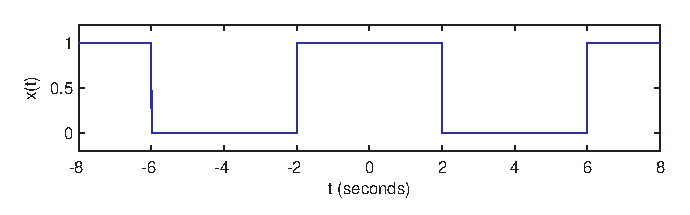
\includegraphics{exrectpulsetrain1}
\end{center}
The signal is periodic.  By inspection the fundamental period is $T = 8$, so the fundamental frequency is $\omega_0 = \frac{2 \pi}{8} = \frac{\pi}{4}$ rad/s.  The signal can therefore be expressed as a Fourier series
\begin{equation*}
  x(t) = \sum_{k=-\infty}^{\infty} a_k e^{j k \omega_0 t} = \sum_{k=-\infty}^{\infty} a_k e^{j k \left( \frac{\pi}{4} \right) t},
\end{equation*}
and the coefficients can be found using the analysis equation
\begin{equation*}
  a_k = \frac{1}{T} \int_{-T/2}^{T/2} x(t) e^{-j k \omega_0 t} dt = \frac{1}{8} \int_{-4}^{4} x(t) e^{-j k \left( \frac{\pi}{4} \right) t} dt.
\end{equation*}
The integration interval $[-4,4]$ corresponds to one complete period and is convenient for this problem.

To evaluate $a_k$ we note that over the integration limits the signal is only nonzero from $-2$ to $2$, and within these limits it has a value of exactly one.  The coefficients are therefore
\begin{align*}
  a_k = \frac{1}{8} \int_{-2}^{2} e^{-j k \left( \frac{\pi}{4} \right) t} dt.
\end{align*}
It usually helps to calculate $a_0$ separately:
\begin{align*}
  a_0 &= \frac{1}{8} \int_{-2}^{2} e^{-j 0 \left( \frac{\pi}{4} \right) t} dt = \frac{1}{8} \int_{-2}^{2} dt = 1/2.
\end{align*}
For $k \neq 0$, the remaining coefficients are given by
\begin{align*}
  a_k &= \frac{1}{8} \int_{-2}^{2} e^{-j k \left( \frac{\pi}{4} \right) t} dt 
  = \frac{1}{8} \left[ \frac{1}{-j k \left( \frac{\pi}{4} \right)} e^{-j k \left( \frac{\pi}{4} \right) t} \right]_{t=-2}^{t=2} 
  = \frac{1}{-j k \left( \frac{\pi}{4} \right) 8} \left[ e^{-j k \left( \frac{\pi}{4} \right) t} \right]_{t=-2}^{t=2} \\
  &= \frac{1}{-j k \left( \frac{\pi}{4} \right) 8} \left( e^{-j k \left( \frac{\pi}{4} \right) 2} - e^{j k \left( \frac{\pi}{4} \right) 2} \right) 
  = \frac{1}{k \pi} \frac{1}{2j} \left( e^{j k \left( \frac{\pi}{4} \right) 2} - e^{-j k \left( \frac{\pi}{4} \right) 2} \right)
  = \frac{\sin(\left( \frac{\pi}{2} \right) k)}{k \pi}.
\end{align*}
Each of these coefficient values is real, which is not typically the case --- it only happens when the signal $x(t)$ is real and even.

As always it is useful to plot results in order to visualise them.  Consider the terms in the Fourier series representation
\begin{equation*}
  x(t) = \sum_{k=-\infty}^{\infty} a_k e^{j k \left( \frac{\pi}{4} \right) t}.
\end{equation*}
Each value of $k$ relates to a frequency $\omega = \left( \frac{\pi}{4} \right) k$, and there is a corresponding coefficient value $a_k$.  Plotting the value of $a_k$ as a function of the related frequency is meaningful.  However, since $a_k$ is generally complex, two plots are needed.  It is easier to interpret magnitude and phase plots, so this is what is commonly done.  A plot of each coefficient verses the corresponding frequency is shown below:
\begin{center}
  \psfrag{w}{\scriptsize $\omega$}
  \psfrag{|ak|}{\scriptsize $|a_k|$}
  \psfrag{ang ak}{\scriptsize $\angle a_k$}
  \psfrag{pi}{\scriptsize $\pi$}
  \psfrag{-pi}{\scriptsize $\!\!-\pi$}
  \psfrag{2 pi}{\scriptsize $2\pi$}
  \psfrag{-2 pi}{\scriptsize $-2 \pi$}
  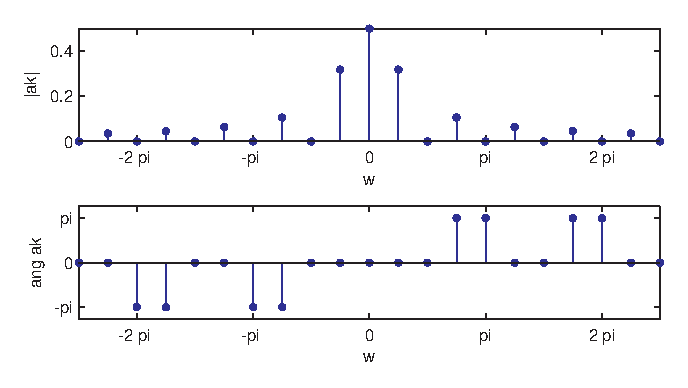
\includegraphics{exrectpulsetrain2}
\end{center}
The term for $k=0$ corresponds to a frequency $\omega = 0$, and the coefficient value is $a_0 = 1/2 = \frac{1}{2} e^{j 0}$.  This is indicated by a dot of value $0.5$ at frequency zero of the magnitude plot, and a dot of value $0$ at the same frequency in the phase plot.  Similarly, $k=1$ corresponds to a frequency $\omega = \frac{\pi}{4}$, for which the coefficient $a_1 = \frac{1}{\pi}$.  Again this is real and positive, so the phase is zero.  The coefficient $a_2 = 0$, which has zero magnitude and any phase --- we have arbitrarily chosen a zero value for the phase, and the point is indicated at $\omega = \frac{\pi}{2}$.  The term for $k=3$ is different.  It corresponds to a frequency $\omega = \frac{3 \pi}{4}$, but the value is $a_3 = -\frac{1}{3 \pi} = \frac{1}{3 \pi} e^{j \pi}$.  The nonzero phase is required to make the value negative, since the magnitude cannot be negative.  The other points can be plotted similarly.

Nonzero points on the negative $\omega$ axis of the phase plot have been indicated with values of $-\pi$.  Since phase is undetermined up to addition of a multiple of $2 \pi$, these points could equally validly have been drawn going upwards rather than downwards.  The reason they are drawn as they are is this:  since
\begin{equation*}
  a_k = \frac{1}{T} \int_{0}^{T} x(t) e^{-j \left( \frac{2 \pi}{T} \right) k t} dt,
\end{equation*}
it is true that
\begin{equation*}
  a_{-k} = \frac{1}{T} \int_{0}^{T} x(t) e^{j \left( \frac{2 \pi}{T} \right) k t} dt
  \quad \text{and} \quad 
  a_{-k}^\ast = \frac{1}{T} \int_{0}^{T} x^\ast(t) e^{-j \left( \frac{2 \pi}{T} \right) k t} dt.
\end{equation*}
If $x(t)$ is real then $x(t) = x^\ast(t)$, and we see from above that it must be true that $a_k = a_{-k}^\ast$.  Writing $a_k = |a_k| e^{j \angle a_k}$ and $a_{-k} = |a_{-k}| e^{j \angle a_{-k}}$, this condition states that for real signals we must have $|a_k| e^{j \angle a_k} = |a_{-k}| e^{-j \angle a_{-k}}$.  Equality of complex numbers means that their magnitudes and phases must be equal, so 
\begin{center}
\fbox{
\begin{minipage}{0.9\textwidth}
For real-valued signals it is always the case that
\begin{equation*}
  |a_k| = |a_{-k}| \qquad \text{and} \qquad \angle a_k = -\angle a_{-k}.
\end{equation*}
The magnitude of the Fourier coefficients is an even function of $k$, and the phase is an odd function.
\end{minipage}
}
\end{center}
For this reason the phase plot in the previous figure was drawn as it was in order to make the phase plot "look" more like an odd function.

It seems evident from the magnitude plot of $|a_k|$ that the coefficient values are tending to zero as $|k| \to \infty$.  This can indeed be shown to be the case.  The nature of the Fourier series representation can therefore be explored by considering the partial reconstruction
\begin{equation*}
  x_N(t) = \sum_{k=-N}^{N} a_k e^{j k \omega_0 t},
\end{equation*}
where the truncated sum means that the reconstruction only uses a subset of the terms in the Fourier series.  We should have $x(t) = \lim_{N \to \infty} x_N(t)$, and indeed this is the case in an appropriately-defined context.  Reconstructed signals for different values of $N$ are shown below:
\begin{center}
  \psfrag{t}{\scriptsize $t$}
  \psfrag{xr2(t)}{\scriptsize $x_2(t)$}
  \psfrag{xr5(t)}{\scriptsize $x_5(t)$}
  \psfrag{xr10(t)}{\scriptsize $x_{10}(t)$}
  \psfrag{xr20(t)}{\scriptsize $x_{20}(t)$}
  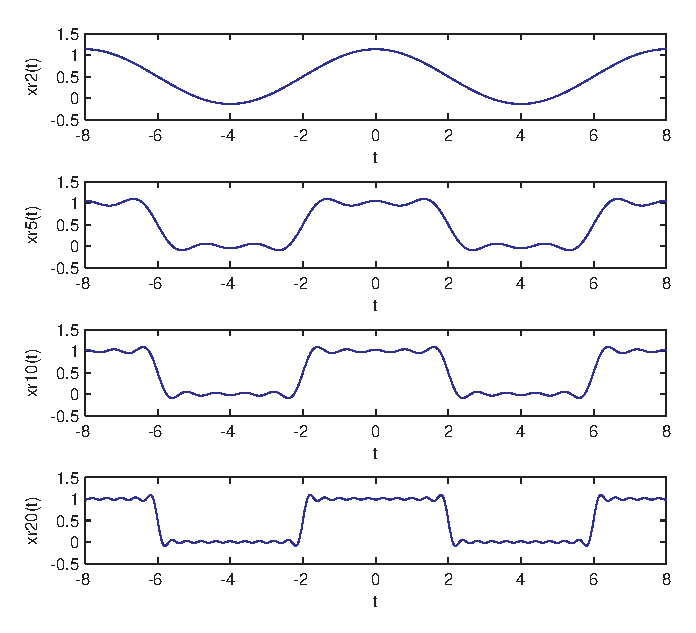
\includegraphics{exrectpulsetrain3}
\end{center}
Small values of $N$ yield a poor reconstruction, but as $N$ increases the reconstructed signal tends towards the original signal $x(t)$. 

In practice one seldom actually reconstructs a signal from its Fourier series coefficients --- it is sufficient just to know that it can be done, and that they completely describe the signal.

\subsection{Example:  impulse train}

One of the most important periodic signals is the {\em impulse train} $p_T(t)$ shown below:
\begin{center}
  \psfrag{t}{\scriptsize $t$}
  \psfrag{pT(t)}{\scriptsize $p_T(t)$}
  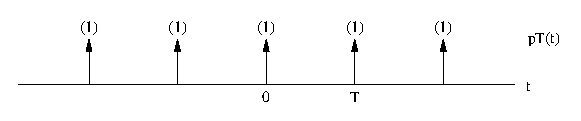
\includegraphics{impulsetrain}
\end{center}
One possible mathematical expression for this signal is
\begin{equation*}
  p_T(t) = \sum_{k=-\infty}^{\infty} \delta(t - kT).
\end{equation*}
One reason for its importance is that if we convolve {\em any} signal with it, then the result will be periodic with a period of $T$.  For example, if we convolve $p_T(t)$ with $x(t)$ below
\begin{center}
  \psfrag{t}{\scriptsize $t$}
  \psfrag{x(t)}{\scriptsize $x(t)$}
  \includegraphics{impulsetrain2}
\end{center}
then the result $y(t) = x(t) \conv p_T(t) $ will be
\begin{center}
  \psfrag{t}{\scriptsize $t$}
  \psfrag{y(t)}{\scriptsize $y(t)$}
  \includegraphics{impulsetrain3}
\end{center}
Mathematically, this follows from (but is not proved by) the linearity and shift invariance of convolution:
\begin{align*}
  y(t) &= x(t) \conv \left( \sum_{k=-\infty}^{\infty} \delta(t - kT) \right)
  = \sum_{k=-\infty}^{\infty} \left( x(t) \conv \delta(t - kT) \right)
  = \sum_{k=-\infty}^{\infty} x(t - kT),
\end{align*}
{\em Show\marginpar{\bf Exercise:} that the signal $y(t)$ as defined above is periodic with a period $T$.}

Having a Fourier series representation of the impulse train is useful.  Firstly, we note that it is clearly periodic with a period of $T$.  It therefore has a representation of the form
\begin{equation*}
  p_T(t) = \sum_{k=-\infty}^{\infty} c_k e^{j k \omega_0 t}
\end{equation*}
for some set of coefficients $c_k$ and $\omega_0 = \frac{2 \pi}{T}$.  The coefficient values are given by
\begin{equation*}
  c_k = \frac{1}{T} \int_{-T/2}^{T/2} p_T(t) e^{-j k \omega_0 k} dt = \frac{1}{T} \int_{-T/2}^{T/2} \delta(t) e^{-j k \omega_0 t} dt
  = \frac{1}{T} \int_{-T/2}^{T/2} \delta(t) dt = \frac{1}{T},
\end{equation*}
where the sifting property was used and the integration interval was chosen to ensure that we didn't try to integrate over "half" of a Dirac delta.  Substituting back into the Fourier series synthesis equation gives the required representation:
\begin{equation*}
  p_T(t) = \sum_{k=-\infty}^{\infty} \frac{1}{T} e^{j k \left( \frac{2 \pi}{T} \right) t}.
\end{equation*}

\subsection{Trigonometric Fourier series}

If the signal $x(t)$ is real, then it seems a little strange that the Fourier series representation requires a linear combination of {\em complex} exponential components.  Shouldn't a real signal have a real-valued decomposition?

The answer is yes:  a real-valued signal can be written as a linear combination of real-valued components at integer multiples of a fundamental frequency.  In a sense, though, the complex decomposition is simpler. 

If $x(t)$ is real, then it has been shown that the Fourier coefficients satisfy $a_{k} = a_{-k}^\ast$.  In general $a_k$ is complex, so we can write it in magnitude-phase form as $a_k = |a_k|e^{j \angle a_k}$.  With this definition it is evident that $a_{-k} = a_k^\ast = (|a_k| e^{j \angle a_k})^\ast = |a_k| e^{-j \angle a_k}$.

Consider the Fourier series reconstruction formula in this case:
\begin{equation*}
  x(t) = \sum_{k=-\infty}^{\infty} a_k e^{j k \omega_0 t} 
  = \cdots + a_{-2} e^{-j 2 \omega_0 t} + a_{-1} e^{-j \omega_0 t} + a_0 
  + a_1 e^{j \omega_0 t} + a_2 e^{j 2 \omega_0 t} + \cdots
\end{equation*}
Pulling out the $k=0$ term this can be written as
\begin{equation*}
  x(t) = a_0 +  \sum_{k=1}^{\infty} (a_k e^{j k\omega_0 t} + a_{-k} e^{-j k \omega_0 t}).
\end{equation*}
Noting that $\cos \theta = \frac{1}{2} (e^{j \theta} + e^{-j \theta})$ we see that
\begin{align*}
  x(t) &= a_0 +  \sum_{k=1}^{\infty} (|a_k|e^{j \angle a_k} e^{j k\omega_0 t} + |a_k| e^{-j \angle a_k} e^{-j k \omega_0 t}) \\
  &= a_0 +  \sum_{k=1}^{\infty} |a_k| (e^{j (k\omega_0 t + \angle a_k)} + e^{-j (k \omega_0 t + j \angle a_k}) \\
  &= a_0 +  \sum_{k=1}^{\infty} 2 |a_k| \frac{1}{2} (e^{j (k\omega_0 t + \angle a_k)} + e^{-j (k \omega_0 t + j \angle a_k}) \\
  &= a_0 +  \sum_{k=1}^{\infty} 2 |a_k| \cos (k\omega_0 t + \angle a_k).
\end{align*}
The component functions in the weighted sum are now real-valued sinusoids.  This form of decomposition is called the {\em trigonometric Fourier series}.

One can develop direct equations for calculating the parameters of the trigonometric Fourier series for real-valued signals.  They look similar to those for the complex exponential case, but are slightly more intricate and harder to remember.  The above analysis shows that in the case where a signal is real, the complex exponential Fourier coefficients have structure that essentially cases cancellation of all the complex parts of the complex exponential components.

\subsection{Parseval's theorem}

A current $I$ through a resistor $R$ dissipates a total power of $P = I^2 R$.  A voltage $V$ across a resistor $R$ results in a power dissipation of $P = V^2/R$.  The important thing to note is that the power dissipated is proportional to the {\em square} of either the current or the voltage.  

The power of a signal $x(t)$ is defined to be the average of its squared values, or its {\em mean square} value.  Formally, this can be calculated as
\begin{equation*}
  P = \lim_{T \to \infty} \frac{1}{T} \int_0^T |x(t)|^2 dt.
\end{equation*}
The limiting process is required because the signal can have infinite duration.  If $x(t)$ is a current, this calculation finds the average power dissipated when the signal is passed through a reference $R=1$ ohm resistor.  If $x(t)$ is a voltage then it finds the average power dissipated when the voltage signal is held across a reference $R=1$ ohm resistor.

If the signal $x(t)$ is periodic, then we can find its mean-square value without using the limit.  The average power of the signal will just be the average power over one cycle:
\begin{equation*}
  P = \frac{1}{T} \int_0^T |x(t)|^2 dt.
\end{equation*}
Given the description of a signal $x(t)$ in the time domain, it is therefore quite simple to calculate the average power.

Parseval's theorem relates power in the time domain to power in the frequency domain, in terms of the Fourier series coefficients.  

\begin{center}
\fbox{
\begin{minipage}{0.9\textwidth}
Assuming that $x(t)$ has a Fourier series representation
\begin{equation*}
  x(t) = \sum_{k=-\infty}^{\infty} a_k e^{j k \omega_0 t},
\end{equation*}
Parseval's theorem states that
\begin{equation*}
  \frac{1}{T} \int_0^T |x(t)|^2 dt = \sum_{k=-\infty}^{\infty} |a_k|^2.
\end{equation*}
\end{minipage}
}
\end{center}

The theorem can be partially justified as follows.  Consider the $k$th term in the Fourier series representation:  it is a signal of the form $x_k(t) = a_k e^{j \omega_0 t}$.  In isolation, this term has an average power of
\begin{align*}
  P_k &= \frac{1}{T} \int_0^T |x_k(t)|^2 dt = \frac{1}{T} \int_0^T x_k(t) x_k^{\ast}(t) dt 
  = \frac{1}{T} \int_0^T a_k e^{j k \omega_0 t} a_k^{\ast} e^{-j k \omega_0 t} dt \\
  &= \frac{1}{T} a_k a_k^{\ast} \int_0^T e^{j k \omega_0 t} e^{-j k \omega_0 t} dt
  = \frac{1}{T} a_k a_k^{\ast} \int_0^T dt = a_k a_k^{\ast} = |a_k|^2,
\end{align*}
where we've used the fact that $|z|^2 = z z^{\ast}$ for any complex number $z$.  Thus the average power in the $k$th component of $x(t)$ is $|a_k|^2$.  Parseval's theorem states that the total power in the signal is the sum of the power in each of the individual components in the Fourier series representation.  (Note that this is only possible because the complex exponentials in the expansion are orthogonal over one period.)

Thus the total power in $x(t)$ can be found either from the time-domain description, or from the Fourier series coefficients.  However, the Fourier coefficients contain more information:  they additionally let you determine the {\em frequencies} at which the power contributions arise.  

In the example of Section~\ref{sec:exrectpulsetrain}, the average signal power can be found in the time domain as follows:
\begin{equation*}
  P = \frac{1}{8} \int_{-4}^4 |x(t)|^2 dt = \frac{1}{8} \int_{-2}^2 1 dt = \frac{4}{8} = \frac{1}{2}.
\end{equation*}
This would be measured in units of power, probably watts.  The same result can be obtained from the magnitude plot of $|a_k|$:  using Parseval's theorem we have
\begin{align*}
  P &= \sum_{k=-\infty}^{\infty} |a_k|^2 
  = \cdots + \frac{1}{(3 \pi)^2} + \frac{1}{(\pi)^2} + \frac{1}{(2)^2} + \frac{1}{(\pi)^2}  + \frac{1}{(3 \pi)^2} + \cdots \\
  &= \frac{1}{4} + \frac{2}{\pi^2} \sum_{k=0}^{\infty} \frac{1}{(2(k+1) - 1)^2} 
  = \frac{1}{4} + \frac{2}{\pi^2} \frac{\pi^2}{8} = \frac{1}{2}.
\end{align*}
(This is far from obvious.)  However, the theorem also tells us where the power is located in terms of frequency.  The  $k=0$ term corresponds to the component of the signal $a_0 e^{j 0 \omega_0 t} = a_0$, which is constant and has frequency zero (i.e. the DC component of the signal).  The power in the signal at frequency $0$ is therefore $|a_0|^2 = \frac{1}{4}$ watts.  Half of the signal power is therefore contained in the DC component.  

The first harmonic corresponds to the fundamental frequency:  the terms for $k=\pm 1$.  The power contained in $a_1 e^{j \omega_0 t}$ is $\frac{1}{\pi^2}$, and the power in the component $a_{-1} e^{-j \omega_0 t}$ is also $\frac{1}{\pi^2}$.  The total power contained in the first harmonic is therefore $\frac{2}{\pi^2}$ watts.  There is no power in the second harmonic, since the Fourier coefficients are zero, but the power in the third harmonic can similarly be shown to be $\frac{2}{9 \pi^2}$ watts.

The partition of power to different frequencies in the signal allows us to interpret the effect of modifying the signal.  Suppose we were to put $x(t)$ through a system that removes the components of the signal above the third harmonic --- this is the operation of a {\em filter}, which will be discussed at length later on.  Such a filter would null the components of the signal corresponding to frequencies $\omega \geq 4 \omega_0$:  the Fourier components at these frequencies would be set to zero by the action of the system.  The remaining nonzero coefficients are then just $\{a_{-3}, a_{-1}, a_0, a_1, a_3\}$, which have an average power of $\frac{1}{9 \pi^2} + \frac{1}{pi^2} + \frac{1}{4} + \frac{1}{pi^2} + \frac{1}{9 \pi^2} = 0.4752$ watts.  The system therefore removes $0.0248$ watts of signal power.  Alternatively, we could say that $0.4752/0.5 = 95.032$\% of the total signal power is contained in the first three harmonics.

\end{document}